%*******************************************************
% Texture Mapping
%*******************************************************
\section{Texture Mapping}

A texture mapping is enabled by setting a texture image to a
\newline \verb|GeometryNode|. This can be done with the following Lua 
command:
\begin{lstlisting}
  set_texture(<filename>)
\end{lstlisting}
This command sets the texture image on the \verb|PhongMaterial| attached to the
\verb|GeometryNode|. 

Texture mapping is implemented by generating $uv$ texture coordinates for each
of the primitives on an intersection. The texture coordinates are then used to
index into the texture map to produce a diffuse colour to be applied to the
intersection point in the lighting calculations. The following subsections
describe the $uv$ generation methods for each of the primitives and the texture
map sampling algorithm.

\subsection{Generating $uv$ Texture Coordinates}

The $uv$ texture coordinates are 2D coordinates with each coordinate having a
value in the range $[0, 1]$. This section will describe how these coordinates
are generated for each of the primitives.

\subsubsection*{Cone}
The texture coordinates for the cone primitive are calculated as follows:
\begin{equation}
\begin{split}
  u &= \frac{acos(Q \cdot \begin{bmatrix} 1.0 & 0.0 & 0.0 \end{bmatrix}^{T})}
  {\pi} \\
  v &= \frac{Q_{z}}{h}
\end{split}
\end{equation}
Where $Q$ is the intersection point on the cone and $h$ is the height of the
cone. Essentially, the $u$ coordinate is the angle of rotation of the vector 
(from the origin to the intersection point) about the $z$-axis divided by $\pi$ 
in order to scale it to the range $[0, 1]$. The $v$ coordinate is calculated by
dividing the $z$ coordinate of the intersection point by the height (since the
cone is aligned along the $z$-axis).

\subsubsection*{Cylinder}
The texture coordinates for the cylinder primitive are generated in a similar
fashion as the cone:
\begin{equation}
\begin{split}
  u &= \frac{acos(\begin{bmatrix} Q_{x} & Q_{y} & 0.0 \end{bmatrix}^{T} \cdot 
  \begin{bmatrix} 1.0 & 0.0 & 0.0 \end{bmatrix}^{T})}{\pi} \\
  v &= \frac{Q_{z}}{h} + 0.5
\end{split}
\end{equation}
Note that the finite cyclinder is defined over $\frac{-h}{2} < z < \frac{h}{2}$,
thus it is necessary to add the $0.5$ term to the $v$ coordinate in order to
produce a value in the range of $[0, 1]$.

\subsubsection*{Disc}
Since the disc lies on the $xy$-plane, the texture coordinates are generated
with the following equation:
\begin{equation}
\begin{split}
  u &= \frac{Q_{x}}{2r} + 0.5 \\
  v &= \frac{Q_{y}}{2r} + 0.5 \\
\end{split}
\end{equation}
Where $r$ is the radius of the disc. The $0.5$ term is added to each coordinate 
since the diameter of the disc ranges from $[-r, r]$.

\subsubsection*{Plane}
Since the bounded plane lies on the $xz$-plane, the texture coordinates are
generated as follows:
\begin{equation}
\begin{split}
  u &= \frac{Q_{x}}{s} + 0.5 \\
  v &= \frac{Q_{z}}{s} + 0.5 
\end{split}
\end{equation}
Where $s$ is the dimension of the plane (width and height are equal). 

\subsubsection*{Torus}
To find the $uv$ coordinates for the torus we first need to define two angles.
\begin{equation}
\begin{split}
  \theta &= asin(\frac{Q_{z}}{r}) \\
  \phi &= asin(\frac{Q_{y}}{r_{0} + r_{1}cos(\theta)})
\end{split}
\end{equation}
Where $r_{0}$ is the major radius and $r_{1}$ is the minor radius. The geometric
representation of the angles are given in Figure~\ref{fig:image3}. Essentially,
$\theta$ is the angle around the tube of the vector from the center of the 
torus' tube to the intersection point. The angle $\phi$ is the radial angle of
the vector from the origin to the intersection point.

\begin{figure}[ht]
  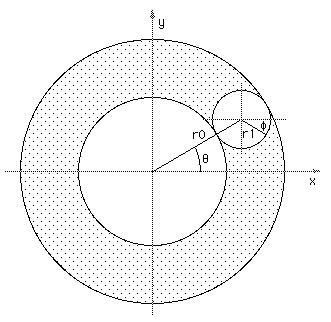
\includegraphics[width=0.5\textwidth, center]{torus}
  \caption{Illustration of the geometric meaning of the angles $\theta$ and 
  $\phi$ (Bourke, 1990).}
  \label{fig:image3}
\end{figure}

Using the two angles we can then generate the $uv$ coordinates as follows:
\begin{equation}
\begin{split}
  u &= \frac{\phi}{\pi} + 0.5 \\
  v &= \frac{\theta}{\pi} + 0.5
\end{split}
\end{equation}

\subsection{Sampling the Texture Map}
Once the $uv$ coordinates are generated, they are used to index into the texture
map to retrieve a colour value:
\begin{equation}
\begin{split}
  i &= \floor*{u(w - 1)} \\
  j &= \floor*{v(h - 1)}
\end{split}
\end{equation}
Where $w$ and $h$ are the width and height of texture map, respectively.

However, this does not produce very nice images since the $uv$ coordinates may
in fact index in between pixels in the texture map. A simple method to solve
this issue is to use bilinear filtering (Blinn \& Newell, 1976). The idea is to
take a weighted average of the surrounding four pixels of the texture coordinate
(Figure~\ref{fig:image4}). The closer the texture coordinate is to a pixel in
the texture map, the larger the weight of that pixel on the final colour.

\begin{figure}[ht]
  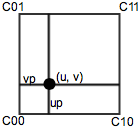
\includegraphics[width=0.5\textwidth, center]{bilinear_filtering}
  \caption{$C_{00}$, $C_{01}$, $C_{10}$, $C_{11}$ represent the colour of the
  surrounding pixels. The area of the four rectangles created by the $uv$ 
  texture coordinate are used as the weights for the colour values.}
  \label{fig:image4}
\end{figure}

Thus, the colour, $C$, can be calculated using bilinear filtering as follows:
\begin{equation}
\begin{split}
  u_{p} &= u(w - 1) - i \\
  v_{p} &= v(h - 1) - j \\
  C &= (1 - u_{p})(1 - v{p})C_{00} + (1 - u_{p})(v_{p})C_{01} + \\
  & (u_{p})(1 - v_{p})C_{10} + (u_{p})(v_{p})C_{11}
\end{split}
\end{equation}

